\documentclass[fleqn]{goose-article}

\title{Energy barrier}
\author{Tom de Geus}
\hypersetup{pdfauthor={T.W.J. de Geus}}

\begin{document}

\maketitle

\section*{Protocol}

The protocol is as follows.
\begin{enumerate}
    \item An element is selected for triggering
    (in the example below chosen in the center of the system).
    Its location is denoted by $\vec{r}'$.

    \item A perturbation around a stress- and strain-free configuration is considered.
    To this end, the selected element (only) is subjected to an eigen stress
    $\bm{\sigma}'$.
    The corresponding equilibrium configuration then constitutes to
    the perturbation that will be used.
    It is characterised by the stress field $\delta \vec{u} (\vec{r})$, and corresponding
    stress $\delta \bm{\sigma} (\vec{r})$
    and strain $\delta \bm{\varepsilon} (\vec{r})$ fields.

    \item Two types of perturbations are considered:
    \begin{itemize}
        \item Simple shear:
        $\bm{\sigma}' = \bm{\sigma}'_s = \vec{e}_x \vec{e}_y + \vec{e}_x \vec{e}_y$.
        Gives: $\delta \vec{u}_s (\vec{r})$, $\delta \bm{\sigma}_s (\vec{r})$, and
        $\delta \bm{\varepsilon}_s (\vec{r})$.

        \item Pure shear:
        $\bm{\sigma}' = \bm{\sigma}'_p = \vec{e}_x \vec{e}_x - \vec{e}_y \vec{e}_y$.
        Gives: $\delta \vec{u}_p (\vec{r})$, $\delta \bm{\sigma}_p (\vec{r})$, and
        $\delta \bm{\varepsilon}_p (\vec{r})$.
    \end{itemize}

    For the triggered element the strain (and) stress are empirically
    of the following structure:
    \begin{itemize}
        \item Simple shear perturbation:
        $\delta \bm{\varepsilon}_s (\vec{r}') = \delta \gamma (\vec{e}_x \vec{e}_y + \vec{e}_x \vec{e}_y)$
        \item Pure shear perturbation:
        $\delta \bm{\varepsilon}_p (\vec{r}') = \delta \mathcal{E} (\vec{e}_x \vec{e}_x - \vec{e}_y \vec{e}_y)$
    \end{itemize}

    \item A perturbation $\Delta \vec{u}(\vec{r}) = s \delta \vec{u}_s (\vec{r}) + p \delta \vec{u}_p (\vec{r})$
    is then applied such that the yield surface is reached in the triggered element in such
    a way that the change in potential energy introduced by the perturbation is minimal.

\end{enumerate}

\begin{figure}[htp]
    \centering
    \captionsetup[subfigure]{justification=centering}
    \begin{minipage}[t]{.49\textwidth}
        \centering
        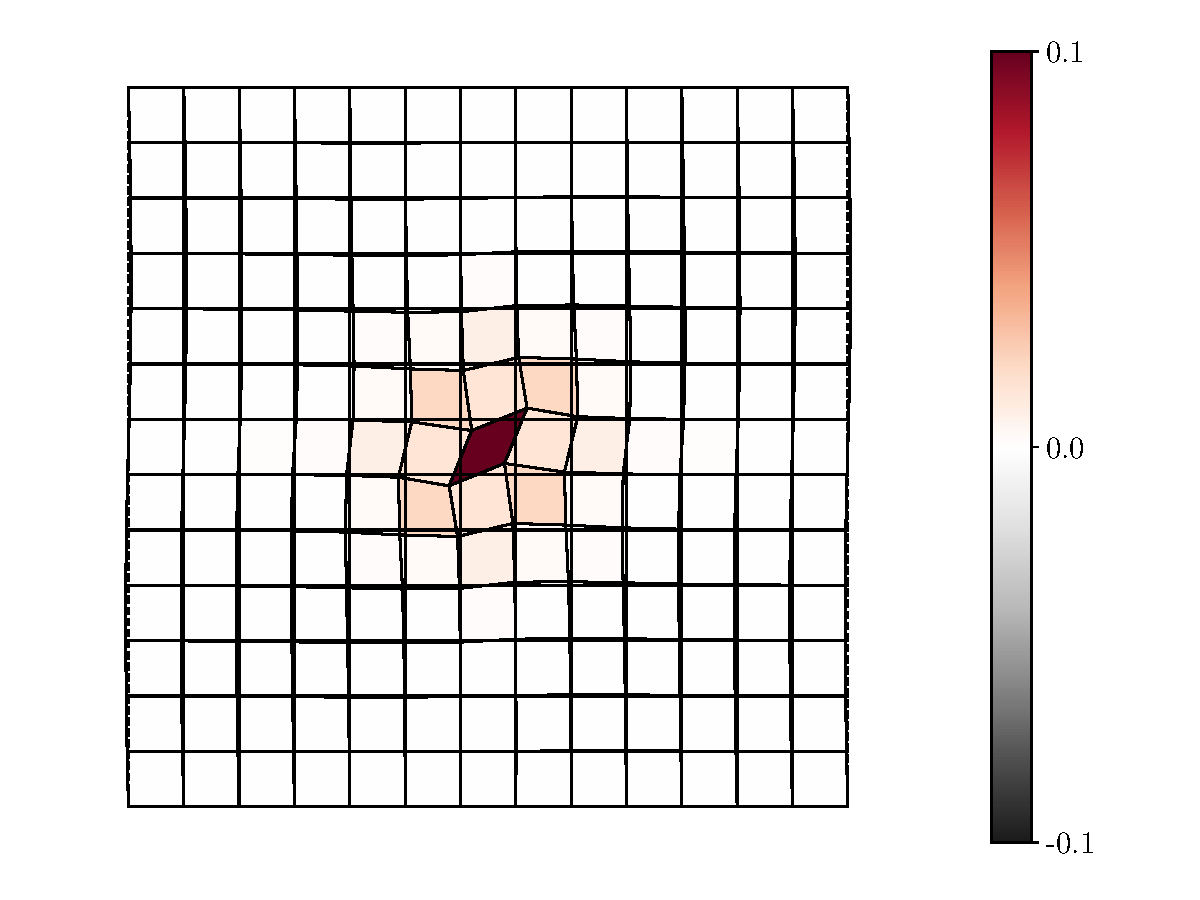
\includegraphics[width=\textwidth]{perturbation_simple-shear_pos.pdf}
        \subcaption{
            Simple shear:
            $\delta \vec{u}_s (\vec{r})$
        }
        \label{fig:perturbation:simple-shear:pos}
    \end{minipage}
    \hfill
    \begin{minipage}[t]{.49\textwidth}
        \centering
        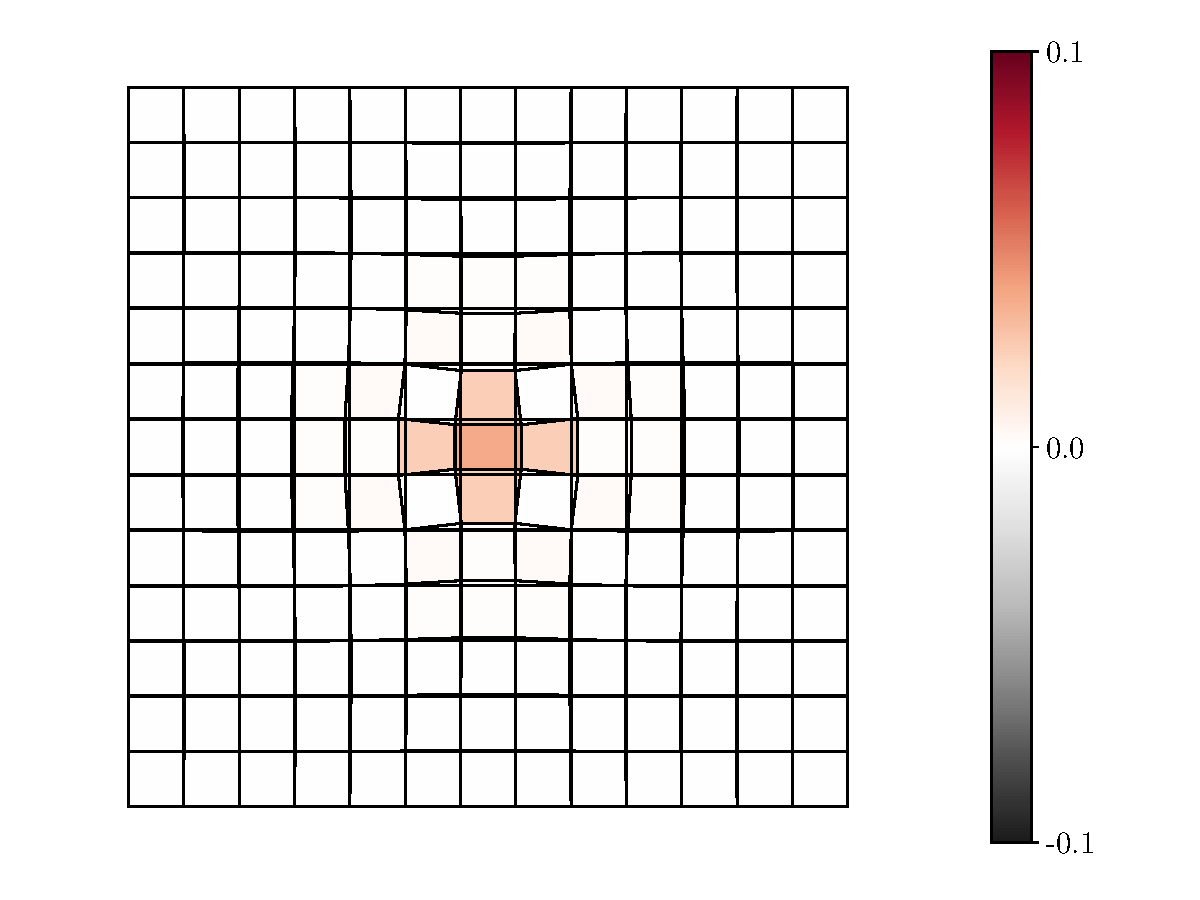
\includegraphics[width=\textwidth]{perturbation_pure-shear_pos.pdf}
        \subcaption{
            Pure shear:
            $\delta \vec{u}_p (\vec{r})$
        }
        \label{fig:perturbation:pure-shear:pos}
    \end{minipage}
    \\
    \begin{minipage}[t]{.49\textwidth}
        \centering
        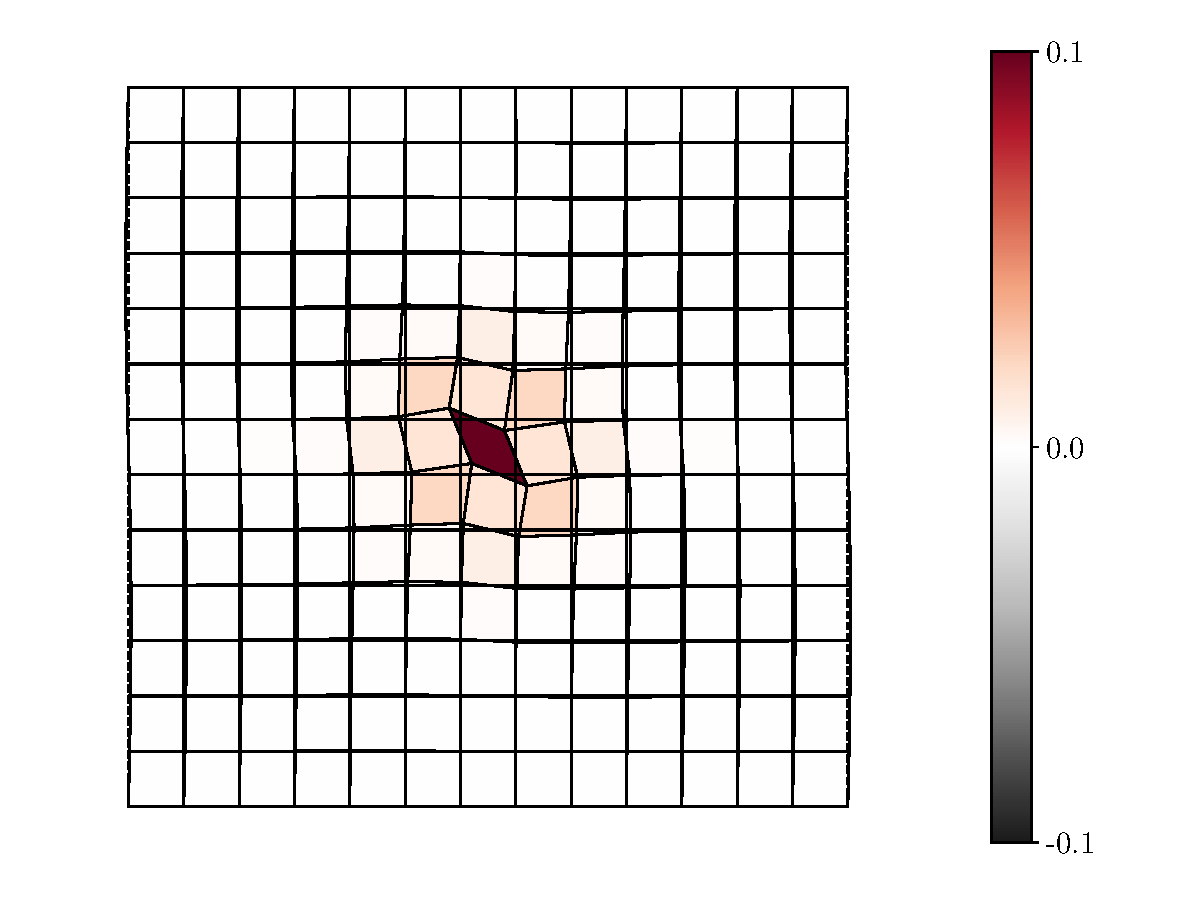
\includegraphics[width=\textwidth]{perturbation_simple-shear_neg.pdf}
        \subcaption{
            Simple shear:
            $- \delta \vec{u}_s (\vec{r})$
        }
        \label{fig:perturbation:simple-shear:neg}
    \end{minipage}
    \hfill
    \begin{minipage}[t]{.49\textwidth}
        \centering
        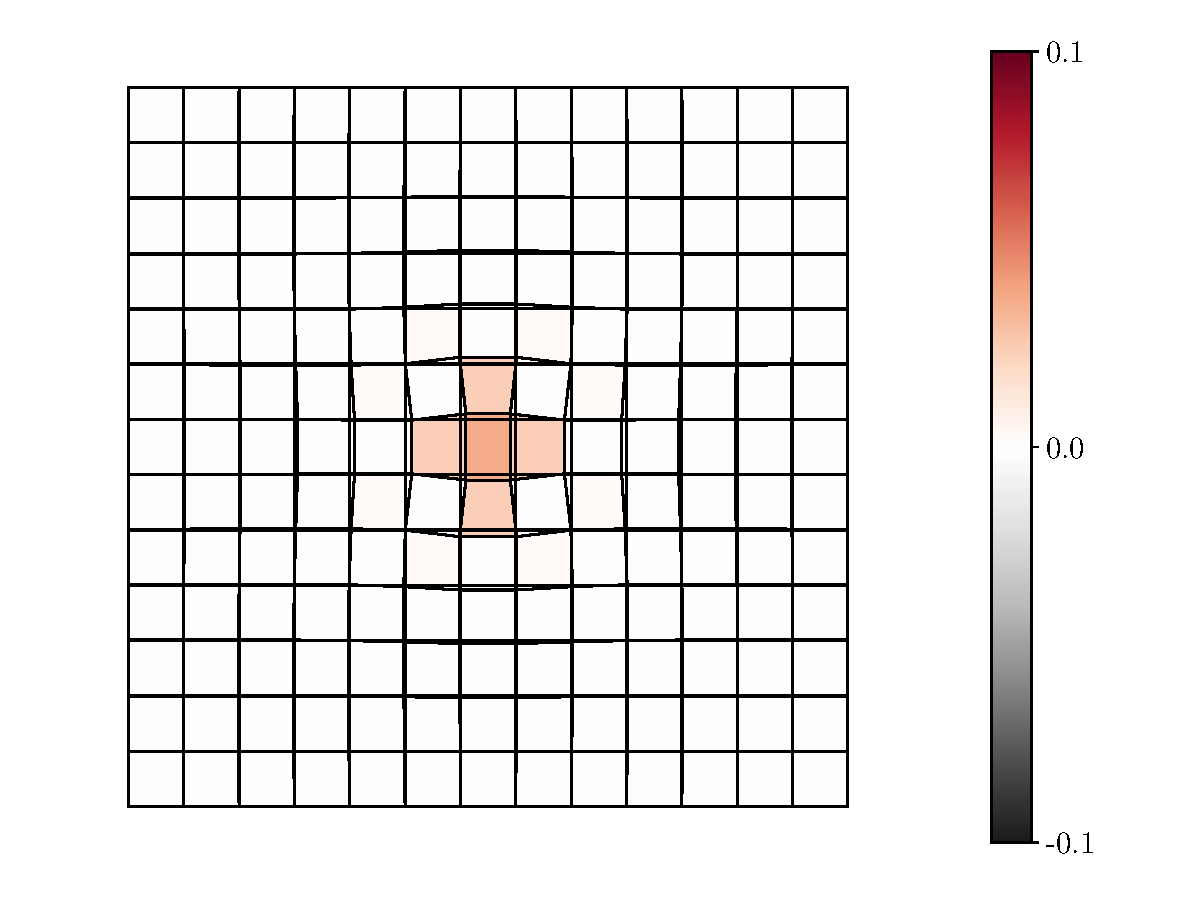
\includegraphics[width=\textwidth]{perturbation_pure-shear_neg.pdf}
        \subcaption{
            Pure shear:
            $- \delta \vec{u}_p (\vec{r})$
        }
        \label{fig:perturbation:pure-shear:neg}
    \end{minipage}
    \caption{
        Perturbation modes.
        The shown colour is the energy change resulting from the perturbation.
    }
    \label{fig:perturbation}
\end{figure}

\begin{figure}[htp]
    \centering
    \begin{minipage}[t]{.49\textwidth}
        \centering
        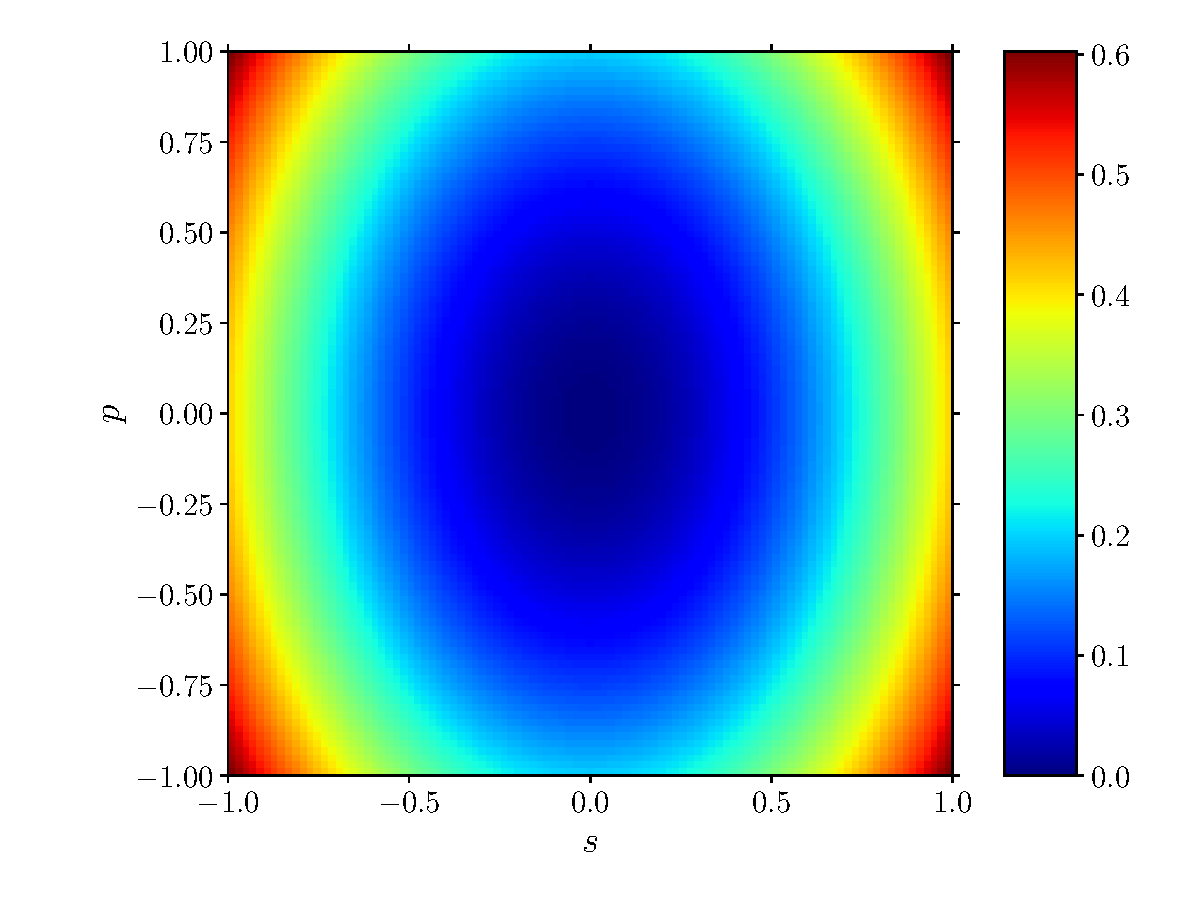
\includegraphics[width=\textwidth]{perturbation_phase-diagram_energy.pdf}
    \end{minipage}
    \hfill
    \begin{minipage}[t]{.49\textwidth}
        \centering
        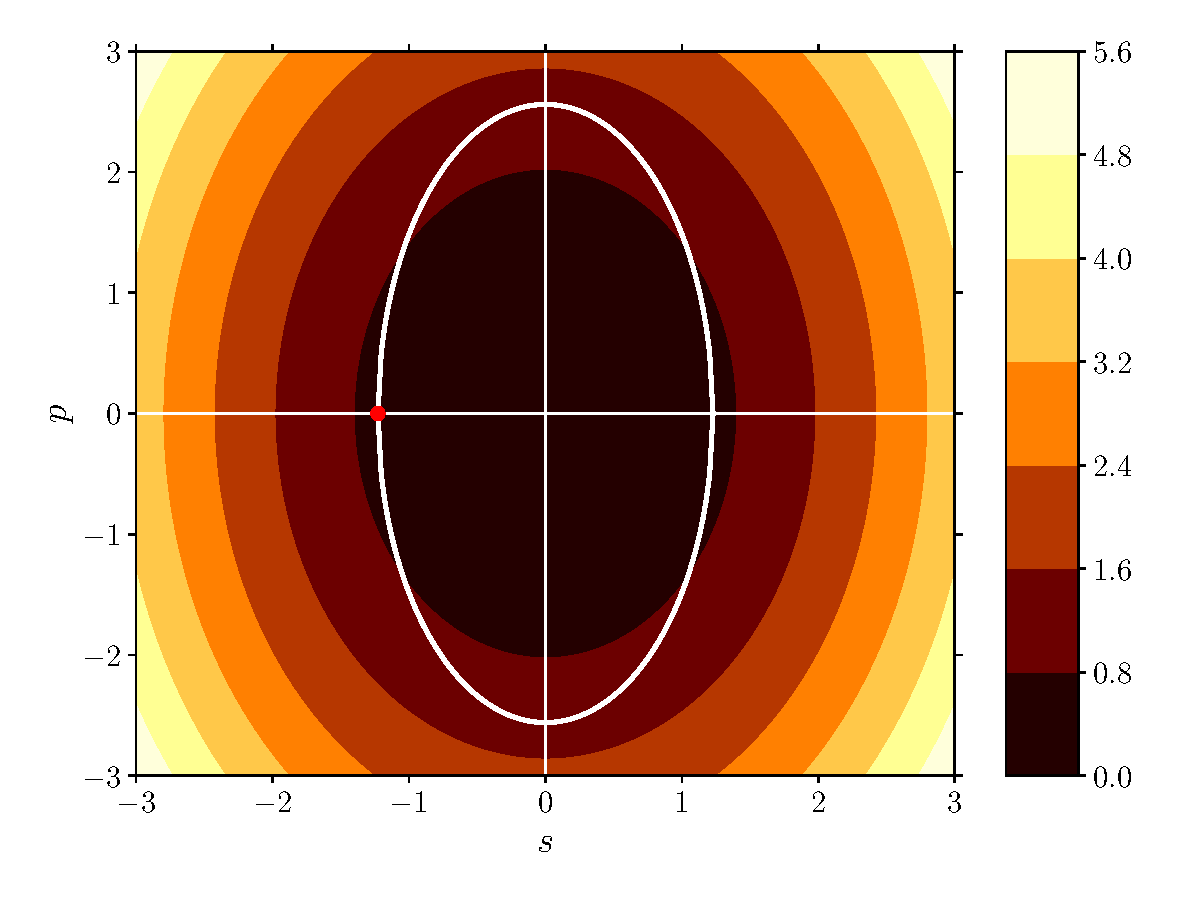
\includegraphics[width=\textwidth]{perturbation_phase-diagram_energy-contour.pdf}
    \end{minipage}
    \caption{
        Change of internal energy, $\Delta E$, for a perturbation:
        $\Delta \vec{u}(\vec{r}) = s \delta \vec{u}_s (\vec{r}) + p \delta \vec{u}_p (\vec{r})$.
        A contour plot is also shown.
    }
    \label{fig:energy}
\end{figure}

\begin{figure}[htp]
    \centering
    \captionsetup[subfigure]{justification=centering}
    \begin{minipage}[t]{.49\textwidth}
        \centering
        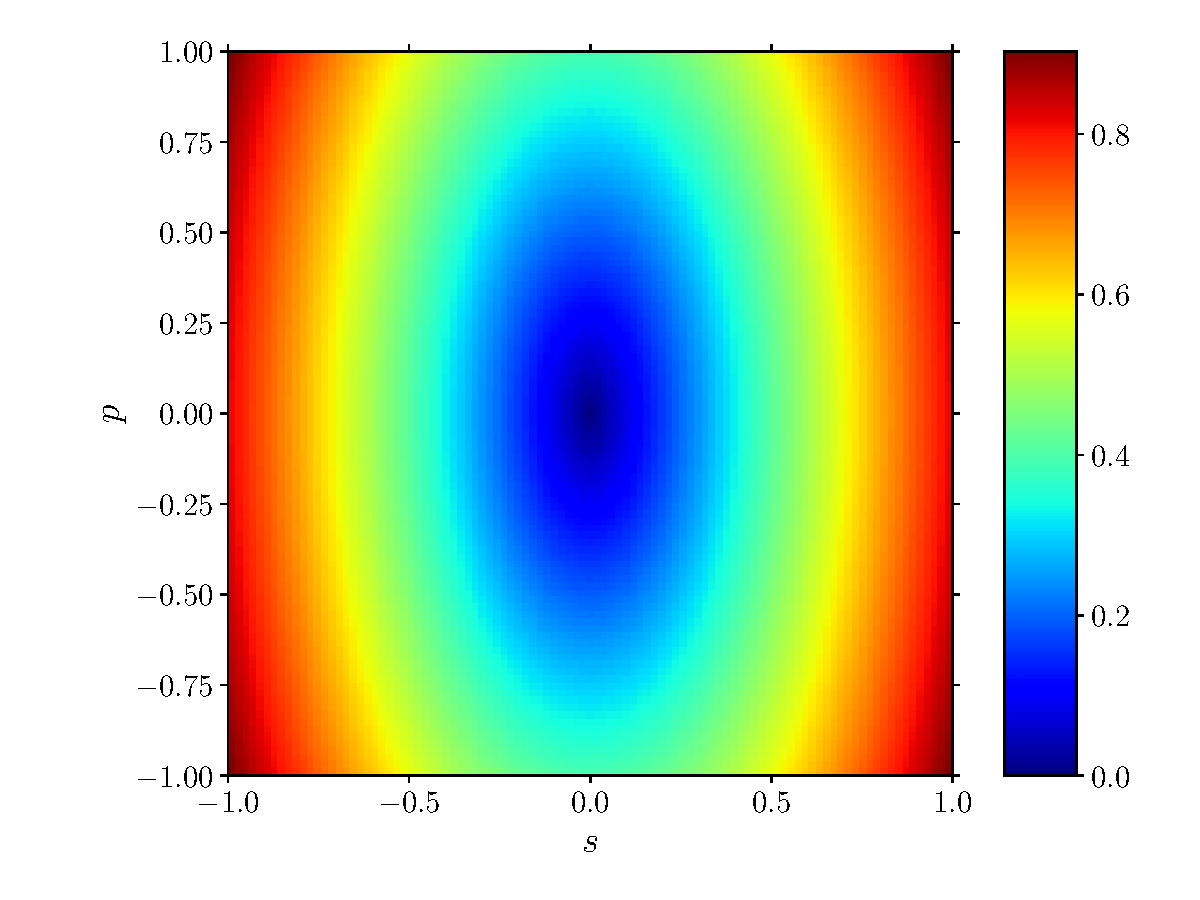
\includegraphics[width=\textwidth]{perturbation_phase-diagram_sig.pdf}
        \subcaption{
            Equivalent stress.
        }
        \label{fig:phase-diagram:sig}
    \end{minipage}
    \hfill
    \begin{minipage}[t]{.49\textwidth}
        \centering
        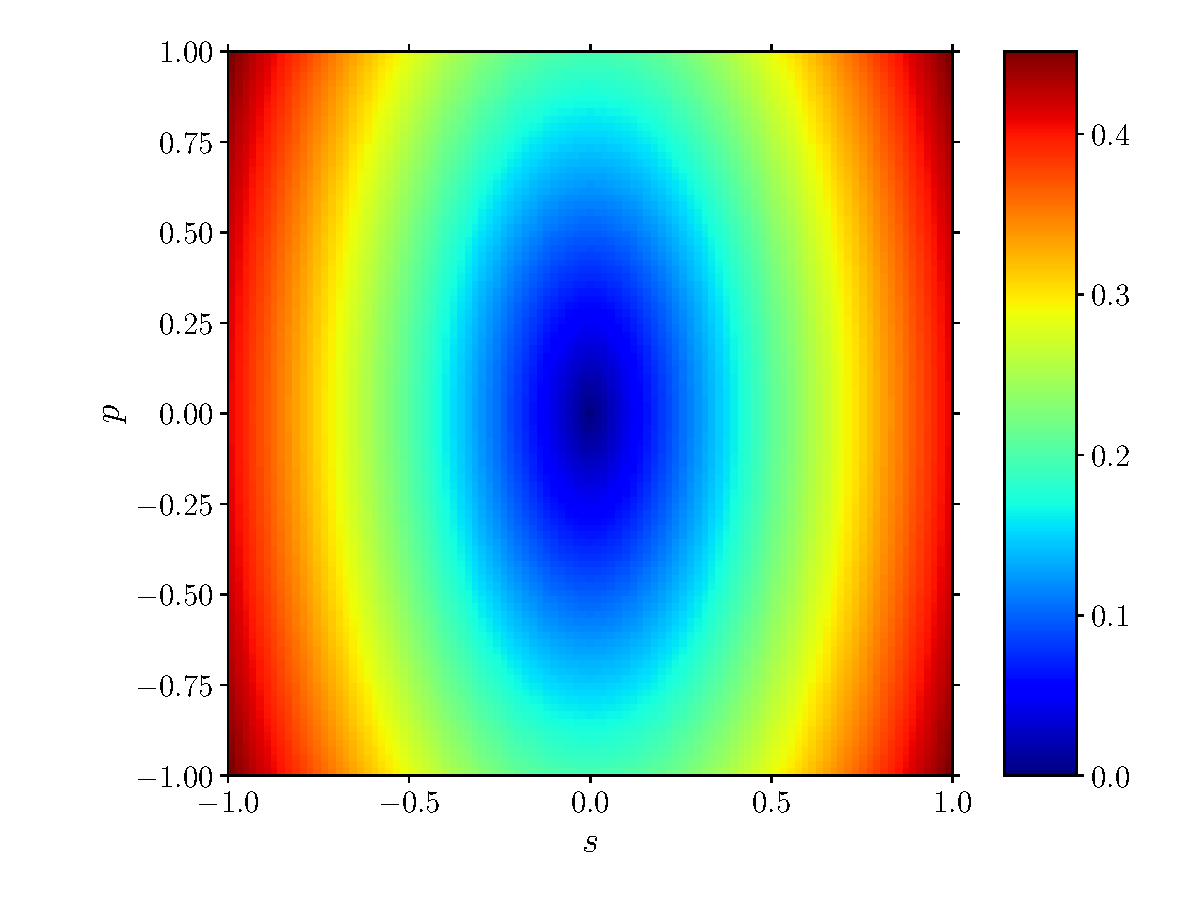
\includegraphics[width=\textwidth]{perturbation_phase-diagram_eps.pdf}
        \subcaption{
            Equivalent strain.
        }
        \label{fig:phase-diagram:eps}
    \end{minipage}
    \caption{
        Resulting
        \subref{fig:phase-diagram:sig} equivalent stress and
        \subref{fig:phase-diagram:eps} equivalent strain
        for a perturbation:
        $\Delta \vec{u}(\vec{r}) = s \delta \vec{u}_s (\vec{r}) + p \delta \vec{u}_p (\vec{r})$.
    }
    \label{fig:phase-diagram}
\end{figure}

\clearpage

\section*{Exploring the yield surface}

\paragraph{Yield surface}

Initially the strain deviator in the triggered element reads
\begin{equation}
    \bm{\varepsilon}_\mathrm{d}(\vec{r}') =
    \begin{bmatrix}
        \mathcal{E} & \gamma \\
        \gamma & - \mathcal{E}
    \end{bmatrix}
\end{equation}
After triggering the strain deviator is
\begin{equation}
    \bm{\varepsilon}_\mathrm{d}^*(\vec{r}') =
    \begin{bmatrix}
        \mathcal{E} + p \delta \mathcal{E} & \gamma + s \delta \gamma \\
        \gamma + s \delta \gamma & - \mathcal{E} - p \delta \mathcal{E}
    \end{bmatrix}
\end{equation}
To reach the yield surface one thus needs to solve
\begin{equation}
    (\mathcal{E} + p \delta \mathcal{E})^2 +
    (\gamma + s \delta \gamma)^2 =
    \varepsilon_y^2
\end{equation}
for $(s, p)$ (with $\varepsilon_y$ the relevant yield strain).

\paragraph{Change of energy}

The energy in the system reads
\begin{equation}
    E = \frac{1}{2} \int_\Omega
        \bm{\sigma}(\vec{r}) : \bm{\varepsilon}(\vec{r})
    \; \mathrm{d} \Omega
\end{equation}
After triggering:
\begin{equation}
    E^* = \frac{1}{2} \int_\Omega
        (\bm{\sigma}(\vec{r}) + \Delta \bm{\sigma}(\vec{r})) :
        (\bm{\varepsilon}(\vec{r}) + \Delta \bm{\varepsilon}(\vec{r}))
    \; \mathrm{d} \Omega
\end{equation}
where
$\Delta \bm{\sigma}(\vec{r}) = s \delta \bm{\sigma}_s(\vec{r}) + p \delta \bm{\sigma}_p(\vec{r})$
and
$\Delta \bm{\varepsilon}(\vec{r}) = s \delta \bm{\varepsilon}_s(\vec{r}) + p \delta \bm{\varepsilon}_p(\vec{r})$.
It is straightforward to show that the change of energy
\begin{equation}
    \Delta E = E^* - E =
    \int_\Omega
        \big(\bm{\sigma}(\vec{r}) + \tfrac{1}{2} \Delta \bm{\sigma}(\vec{r}) \big) :
        \Delta \bm{\varepsilon}(\vec{r})
    \; \mathrm{d} \Omega
\end{equation}
whereby in practice integration is performed numerically, e.g.\
\begin{equation}
    \Delta E = E^* - E =
    \sum\limits_q
        \delta \Omega_q \;
        \big(\bm{\sigma}_q + \tfrac{1}{2} \Delta \bm{\sigma}_q \big) :
        \Delta \bm{\varepsilon}_q
\end{equation}

\clearpage

\section*{Example}

Two examples are included:
A homogeneous medium that is subjected to shear in \cref{fig:example:shear}, and
the same problem additionally subjected to a vertical perturbation
of the top and bottom boundaries \cref{fig:example:prestress}.

\begin{figure}[htp]
    \centering
    \captionsetup[subfigure]{justification=centering}
    \begin{minipage}[t]{.40\textwidth}
        \centering
        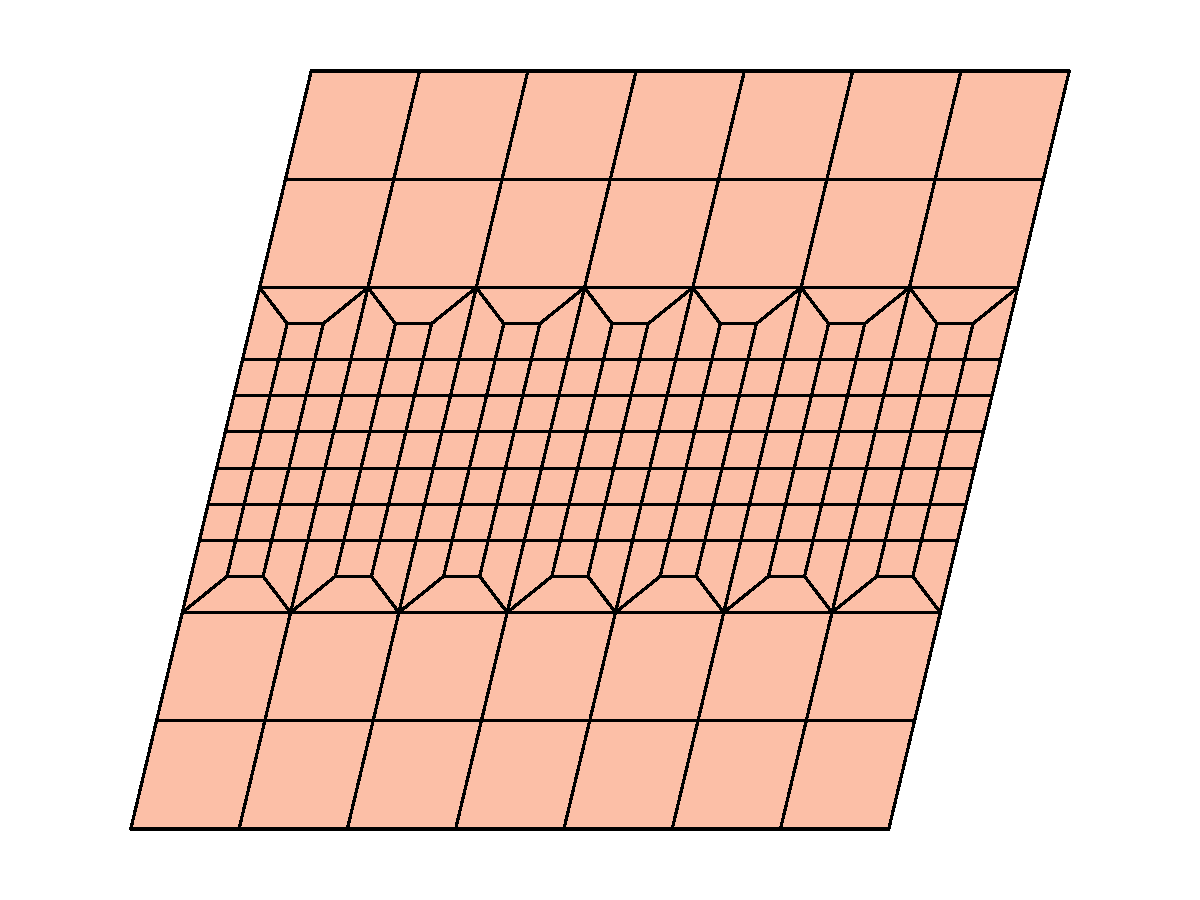
\includegraphics[width=\textwidth]{example_shear_config.pdf}
        \subcaption{Initial configuration.}
    \end{minipage}
    \hspace{0.01\textwidth}
    \begin{minipage}[t]{.40\textwidth}
        \centering
        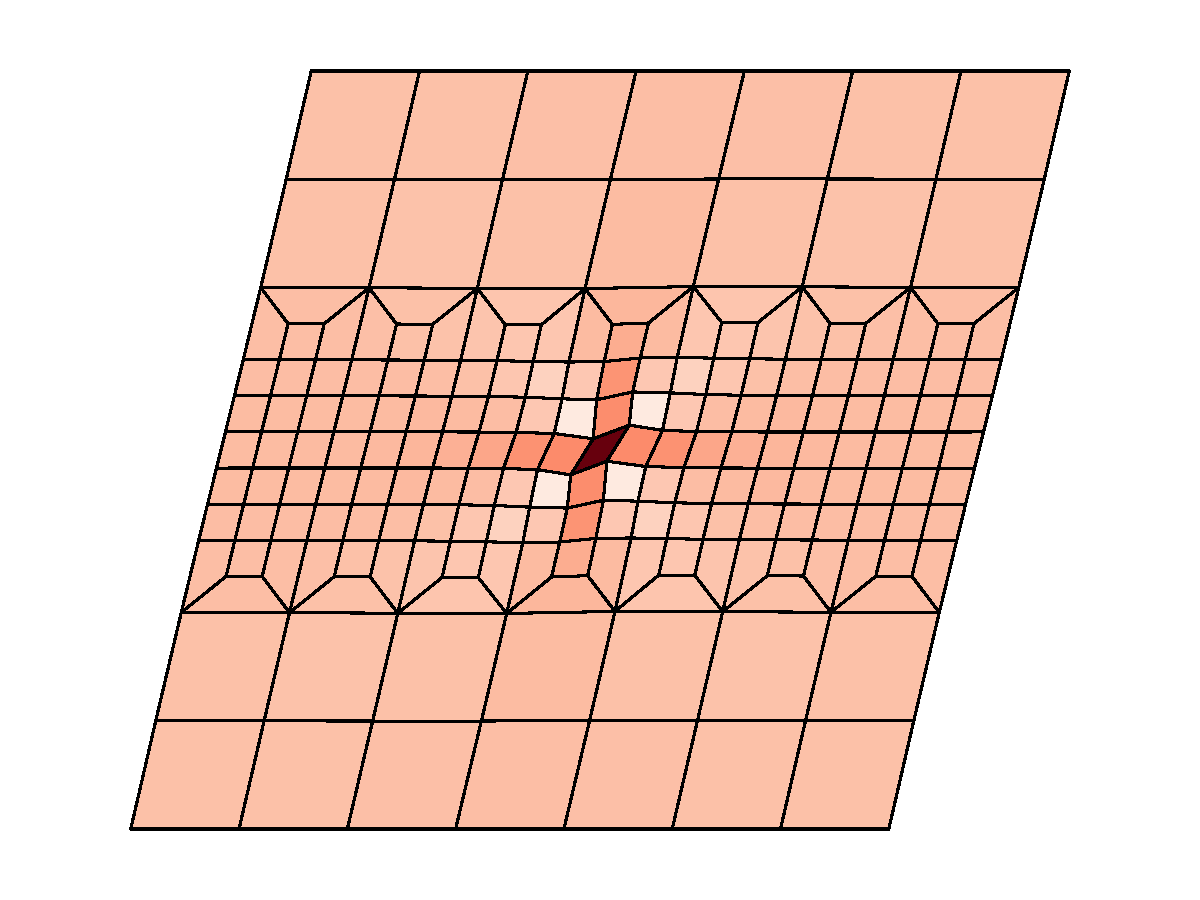
\includegraphics[width=\textwidth]{example_shear_config-perturbed.pdf}
        \subcaption{After perturbation.}
    \end{minipage}
    \\
    \begin{minipage}[t]{.31\textwidth}
        \centering
        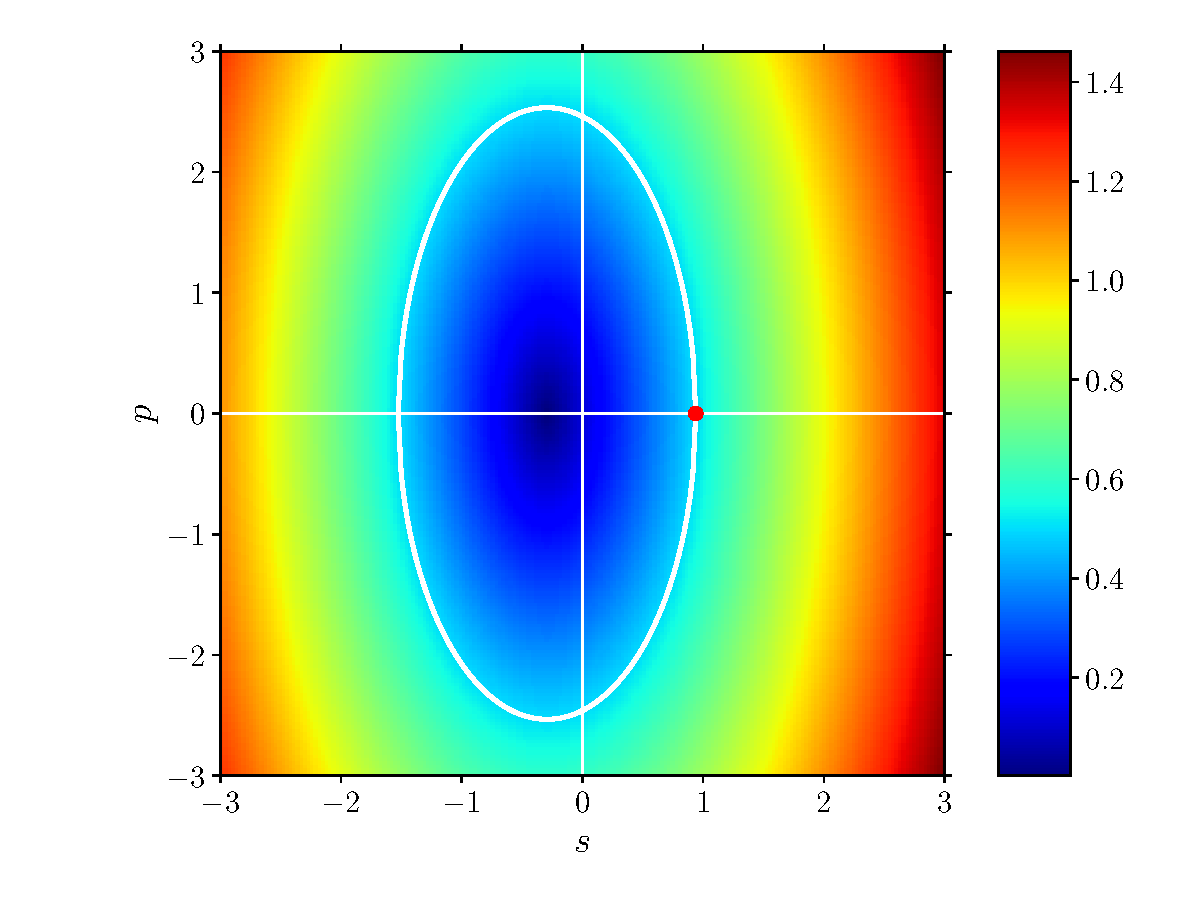
\includegraphics[width=\textwidth]{example_shear_phase-diagram_eps.pdf}
        \subcaption{$\varepsilon$}
    \end{minipage}
    \hfill
    \begin{minipage}[t]{.31\textwidth}
        \centering
        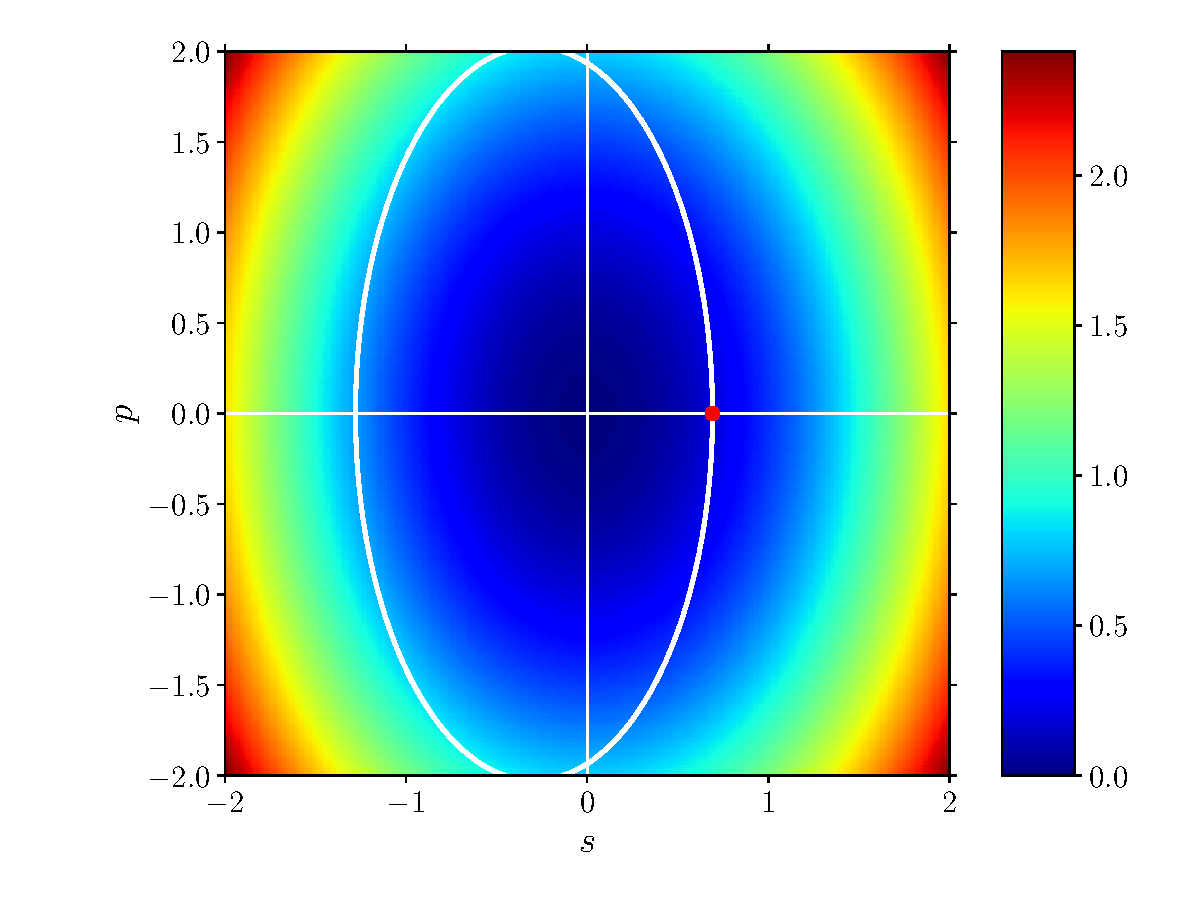
\includegraphics[width=\textwidth]{example_shear_phase-diagram_energy.pdf}
        \subcaption{$\Delta E$}
    \end{minipage}
    \hfill
    \begin{minipage}[t]{.31\textwidth}
        \centering
        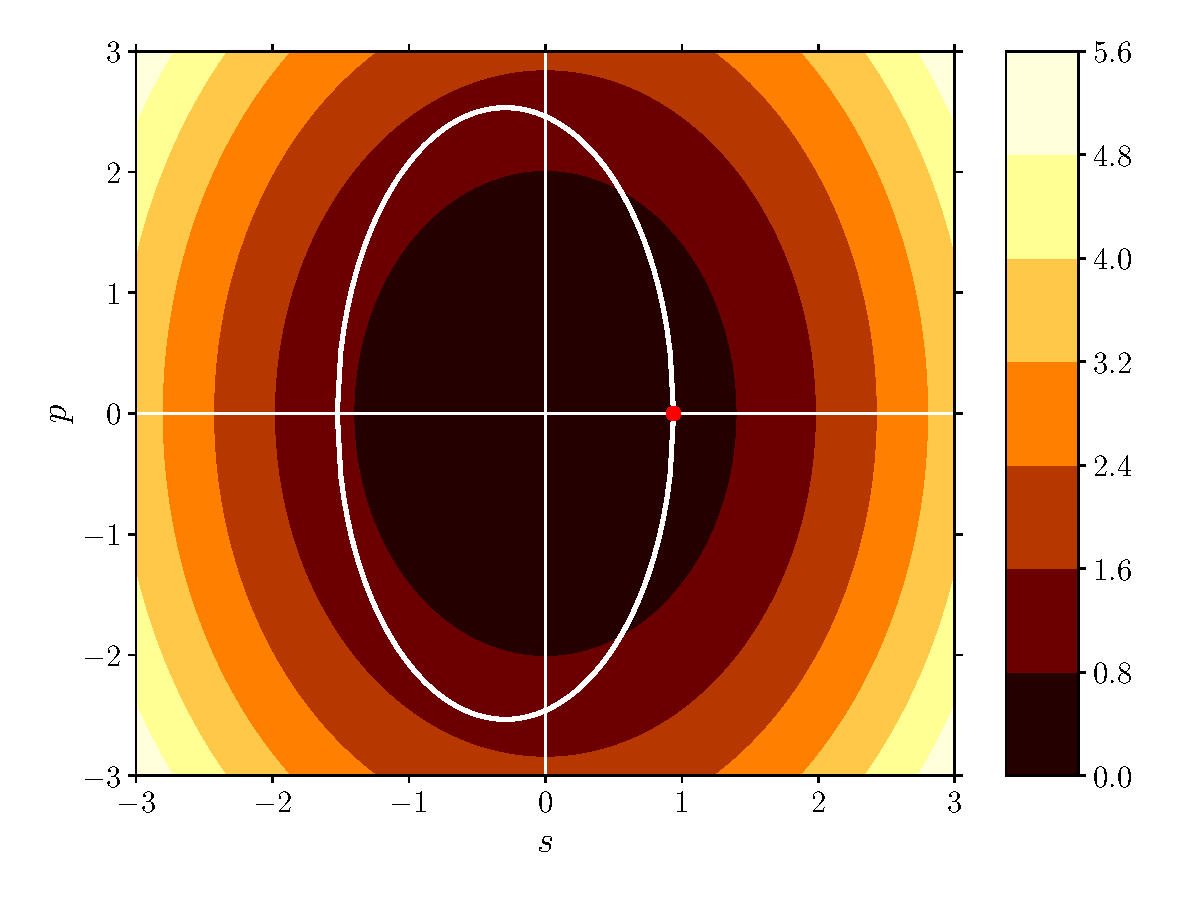
\includegraphics[width=\textwidth]{example_shear_phase-diagram_energy-contour.pdf}
        \subcaption{$\Delta E$}
    \end{minipage}
    \caption{
        (a--b) Starting and perturbed configuration for a homogeneous sheared system.
        (c--e) Phase diagram of a perturbation
        $\Delta \vec{u}(\vec{r}) = s \delta \vec{u}_s (\vec{r}) + p \delta \vec{u}_p (\vec{r})$
        of the configuration in (a).
        The perturbation is applied based on $(s, p)$ that lie on the yield surface and
        that minimise the increase in potential
        energy, as shown using a red dot.
    }
    \label{fig:example:shear}
\end{figure}

\begin{figure}[htp]
    \centering
    \captionsetup[subfigure]{justification=centering}
    \begin{minipage}[t]{.40\textwidth}
        \centering
        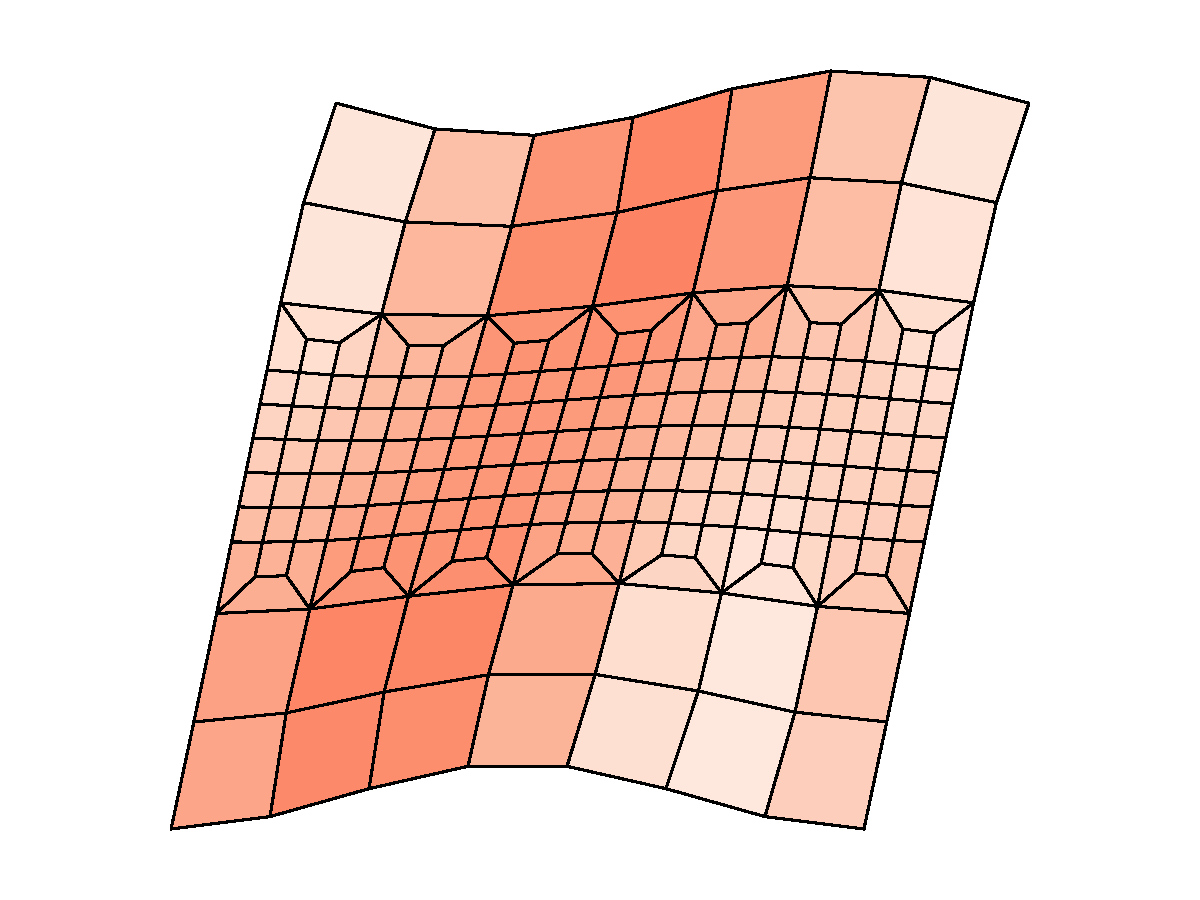
\includegraphics[width=\textwidth]{example_prestress_config.pdf}
        \subcaption{Initial configuration.}
    \end{minipage}
    \hspace{0.01\textwidth}
    \begin{minipage}[t]{.40\textwidth}
        \centering
        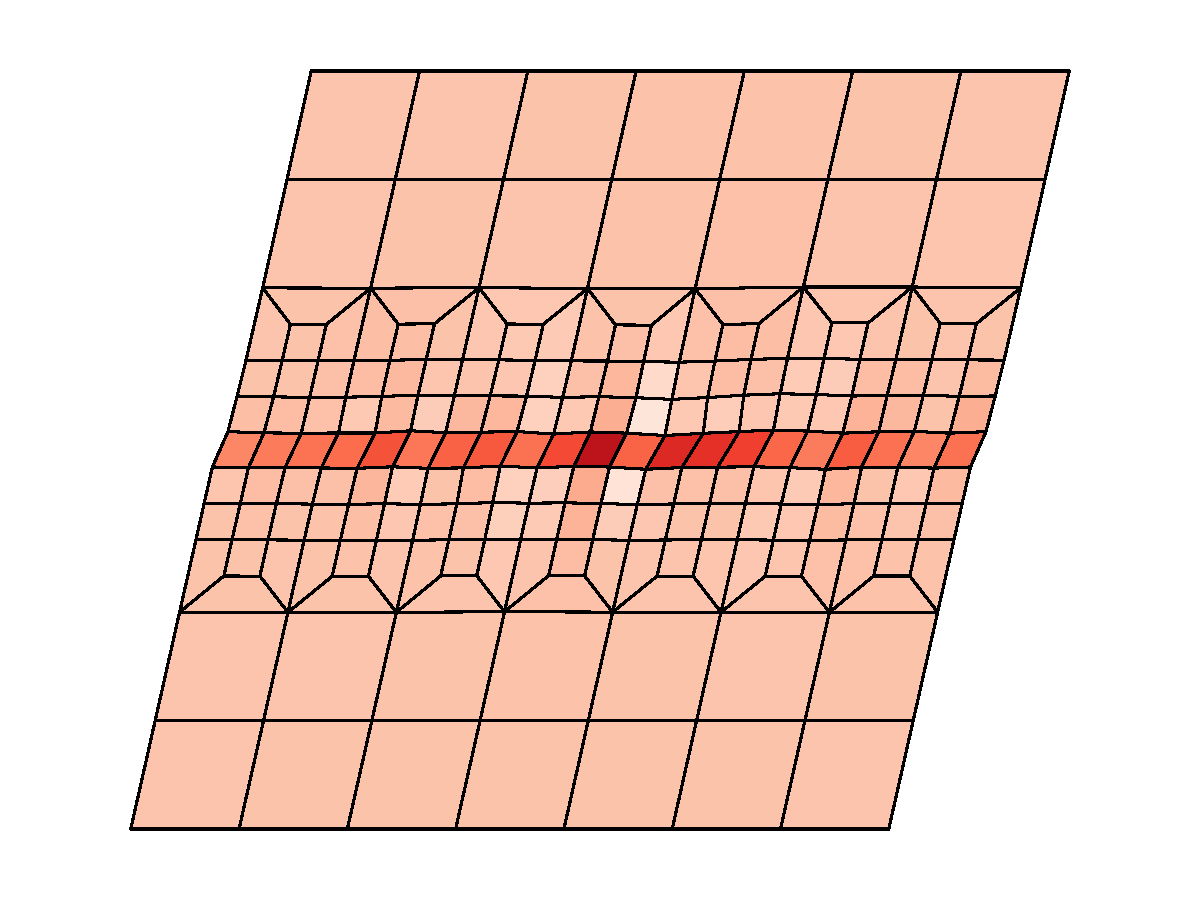
\includegraphics[width=\textwidth]{example_prestress_config-perturbed.pdf}
        \subcaption{After perturbation.}
    \end{minipage}
    \\
    \begin{minipage}[t]{.31\textwidth}
        \centering
        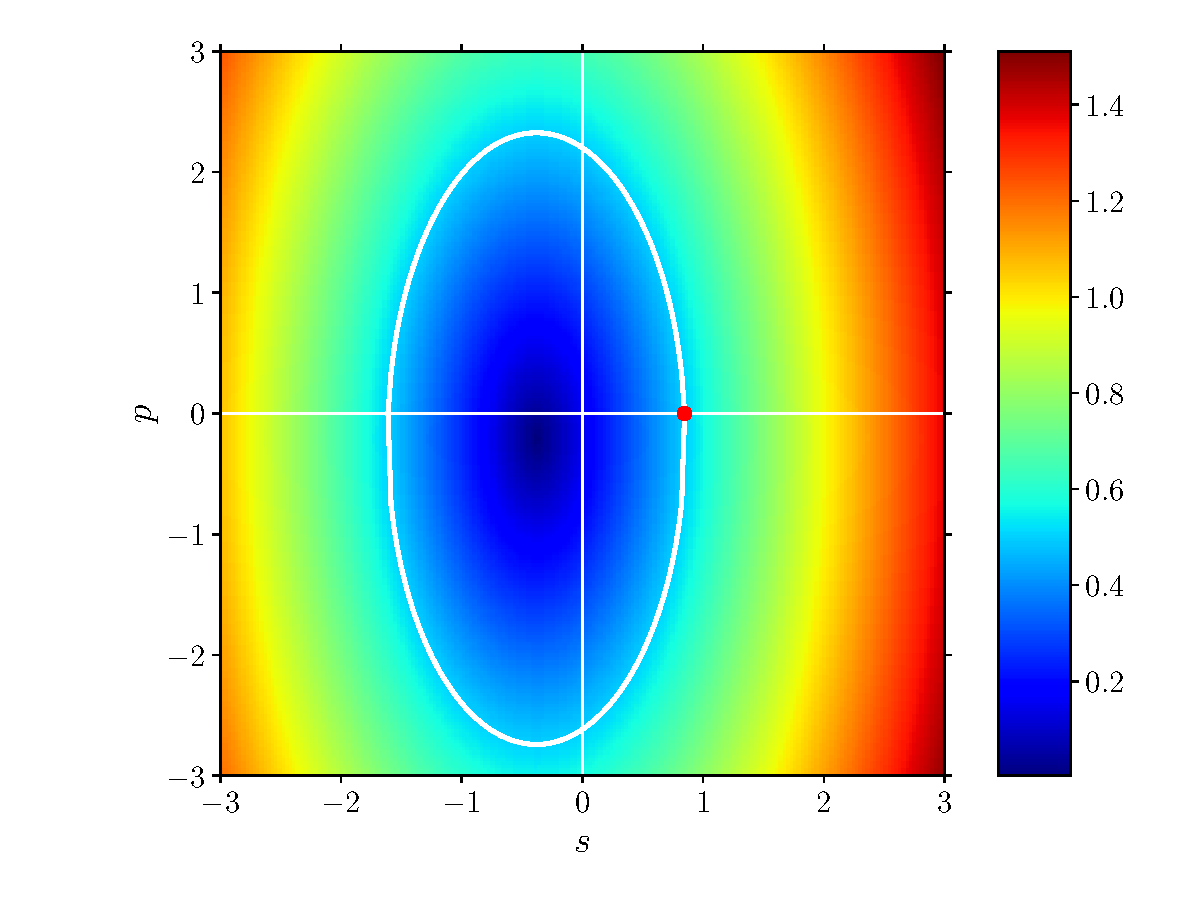
\includegraphics[width=\textwidth]{example_prestress_phase-diagram_eps.pdf}
        \subcaption{$\varepsilon$}
    \end{minipage}
    \hfill
    \begin{minipage}[t]{.31\textwidth}
        \centering
        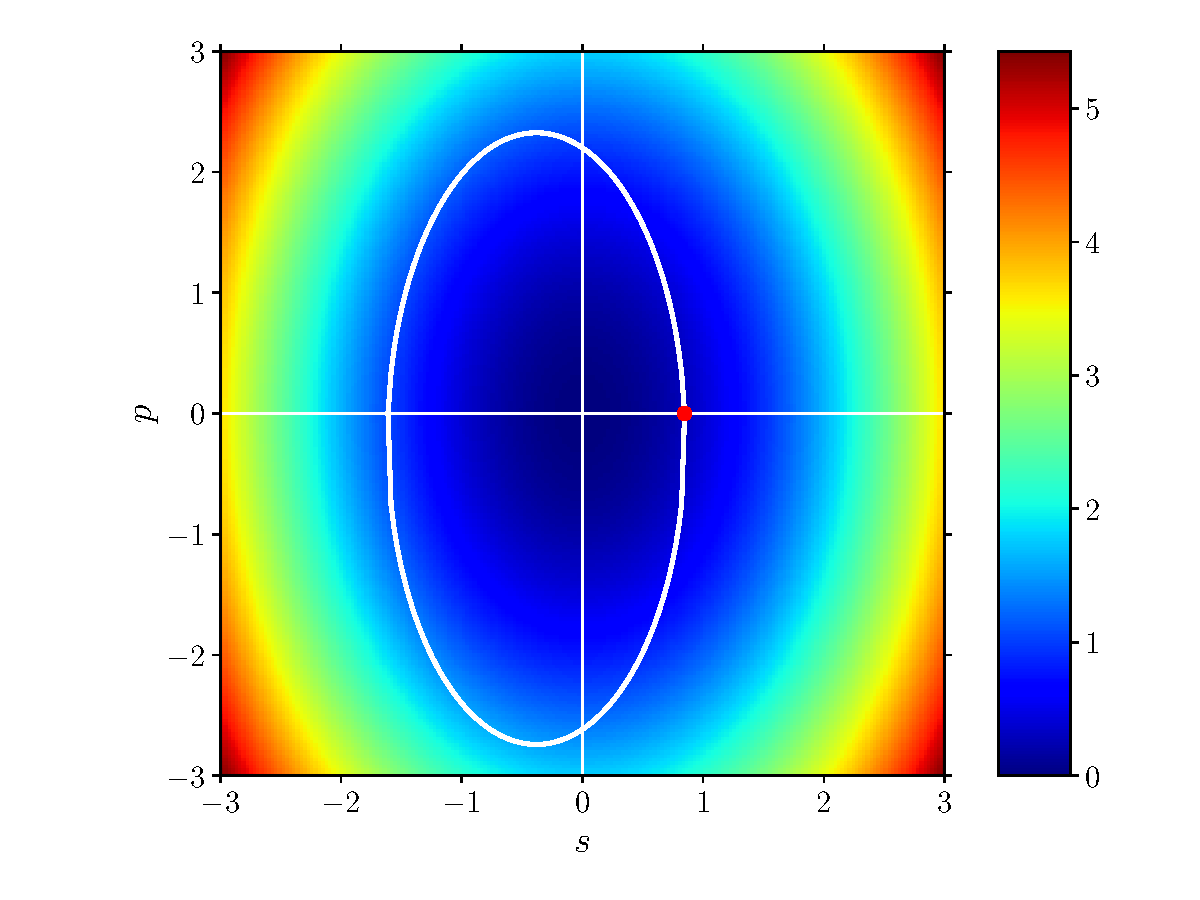
\includegraphics[width=\textwidth]{example_prestress_phase-diagram_energy.pdf}
        \subcaption{$\Delta E$}
    \end{minipage}
    \hfill
    \begin{minipage}[t]{.31\textwidth}
        \centering
        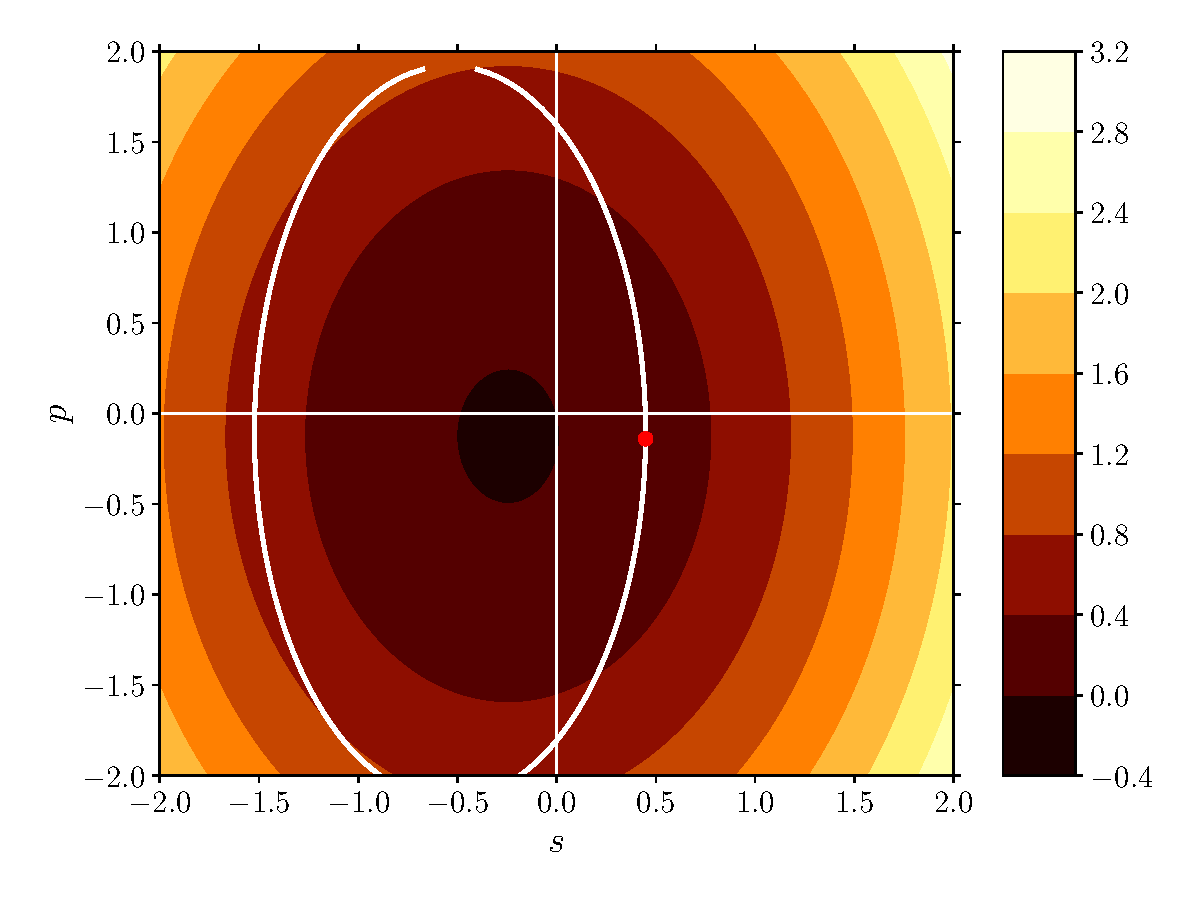
\includegraphics[width=\textwidth]{example_prestress_phase-diagram_energy-contour.pdf}
        \subcaption{$\Delta E$}
    \end{minipage}
    \caption{
        (a--b) Starting and perturbed configuration for a homogeneous sheared system.
        (c--e) Phase diagram of a perturbation
        $\Delta \vec{u}(\vec{r}) = s \delta \vec{u}_s (\vec{r}) + p \delta \vec{u}_p (\vec{r})$
        of the configuration in (a).
        The perturbation is applied based on $(s, p)$ that lie on the yield surface and
        that minimise the increase in potential
        energy, as shown using a red dot.
    }
    \label{fig:example:prestress}
\end{figure}


\end{document}
